%%% -*- TeX-engine: xetex -*-
\documentclass{beamer}

% for themes, etc.
\usepackage{times}  % fonts are up to you
\usepackage{graphicx}
\usepackage{color}
\usepackage{hyperref}

\mode<presentation>
{
  \usetheme{Warsaw}
  \useoutertheme{infolines}
  \usecolortheme{whale}
  \setbeamertemplate{navigation symbols}{}
}
\usepackage{fontspec}
\usepackage{xunicode}
\usepackage[BoldFont,SlantFont]{xeCJK}
\setCJKmainfont{SimSun}
\setCJKmonofont{SimHei}

\title{
  基于翻译技术的流量调度研究 \\
  结题报告
}
\author{王文鑫}
\date{2016年6月8日}

\setbeamertemplate{caption}{\raggedright\insertcaption\par}

\begin{document}

\begin{frame}
  \titlepage
\end{frame}

\section{研究课题}

\begin{frame}
  \frametitle{研究课题}

  \begin{block}{IPv4}
  在IPv4/IPv6过渡场景中,基于翻译等过渡技术,\\设计和实现灵活通用的流量调度机制,\\
  使得ISP可以自由定制多出口情景下的调度策略
  \end{block}
\end{frame}

\section{研究背景}
\subsection{IPv4/IPv6过渡}
\begin{frame}
  \frametitle{IPv4和IPv6}

  \begin{block}{IPv4}
    \begin{itemize}
    \item 地址数量有限:$2^{32} \doteq 43$亿地址,已于2011年2月3日枯竭\footnotemark[1]
    \end{itemize}
  \end{block}

  \begin{block}{IPv6:吸取了IPv4的经验和教训}
    \begin{itemize}
    \item 地址数量巨大:$2^{128} \doteq 10^{38}$个地址
    \item 简化数据格式、配置和路由表,提高效率:
      \begin{itemize}
      \item IP包头:去除了校验码等信息,提高处理效率
      \item 地址配置:利用设备标识自动配置全局可达地址,简化管理
      \item 全局路由表:采用高度聚类的前缀分配原则,提高路由匹配效率
      \end{itemize}
    \item 原生的多播支持、端到端透明、强制IPSec支持……
    \end{itemize}
  \end{block}
  \footnotetext[1]{https://www.nro.net/news/ipv4-free-pool-depleted}
\end{frame}

\begin{frame}
  \frametitle{过渡技术}

  \begin{block}{IPv6不兼容IPv4}
    \begin{itemize}
    \item IPv4到IPv6的切换是一个渐进的过程
      \begin{itemize}
      \item IPv6诞生20周年:扩展迅速,全球覆盖率未过半\footnotemark[1]
      \end{itemize}
    \item 在很长的一段时间内,IPv4和IPv6网络共存
    \end{itemize}
  \end{block}
  \begin{block}{过渡技术}
    \begin{itemize}
    \item 保证升级过程中对原始IPv4应用的支持
    \item 跨越不同IP协议访问网络资源
    \end{itemize}
  \end{block}
  \footnotetext[1]{https://www.google.com/intl/en/ipv6/statistics.html}
\end{frame}

\begin{frame}
  \frametitle{双栈、封装和翻译}

  \vspace{-1em}
  \begin{columns}[T] % align columns
    \begin{column}{.29\textwidth}
      \begin{block}{双栈}
        \begin{itemize}
        \item 不互通的两个协议栈
        \item IPv4地址短缺
        \end{itemize}
      \end{block}
    \end{column}
    \hfill
    \begin{column}{.70\textwidth}
    \end{column}
  \end{columns}
  \begin{columns}[T]
    \begin{column}{.29\textwidth}
      \begin{block}{封装}
        \begin{itemize}
        \item 一种IP协议数据包封装另一种
        \item 协议不互通
        \end{itemize}
      \end{block}
    \end{column}
    \hfill
    \begin{column}{.70\textwidth}
    \end{column}
  \end{columns}
  \begin{columns}[T]
    \begin{column}{.29\textwidth}
      \begin{block}{翻译}
        \begin{itemize}
        \item 对IP包头进行翻译协议
        \item 协议间互通
        \end{itemize}
      \end{block}
    \end{column}
    \hfill
    \begin{column}{.70\textwidth}
    \end{column}
  \end{columns}
\end{frame}

\begin{frame}
  \frametitle{课题研究的过渡场景}

  \begin{block}{使用IPv6主干网承载IPv4端到端通信}
    \begin{itemize}
    \item 用户端和资源端均存在大量不支持IPv6协议的应用
    \item ISP的IPv6网络越来越成熟
    \item 翻译技术:DIVI、NAT64
    \item 封装技术:DS-Lite
    \end{itemize}
  \end{block}
\end{frame}

\begin{frame}
  \frametitle{DIVI、NAT64、DS-Lite}

\end{frame}

\subsection{多出口流量调度}
\begin{frame}
  \frametitle{多出口流量调度}

  \begin{block}{多出口的作用}
    \begin{itemize}
    \item 优化带宽利用率、成本,主备切换……
    \item 搭建不同过渡系统,优势互补
    \item 按照一定的策略引导用户流量进入不同的上游网络
    \end{itemize}
  \end{block}

  \begin{block}{调度机制}
    \begin{itemize}
    \item 传统IPv4网络:BGP、策略路由
    \item 过渡场景:用户的IPv4流量先在用户接入口汇聚
    \item 将流量导向不同的过渡系统,从而选择上游出口
    \end{itemize}
  \end{block}
\end{frame}

\subsection{课题工作内容}
\begin{frame}
  \frametitle{工作内容}

  \begin{block}{工作}
    \begin{itemize}
    \item 调度机制设计和实现
      \begin{itemize}
      \item 灵活:基于五元组
      \item 通用:与具体过渡技术解耦
      \end{itemize}
    \item 修改现有过渡技术,适配多出口场景
    \item 测试和验证
    \end{itemize}
  \end{block}

  \begin{block}{意义}
    \begin{itemize}
    \item 使得过渡场景下的流量调度应用设计和开发成为可能
    \item ISP通过制定调度策略,优化用户体验和管理成本
    \end{itemize}
  \end{block}
\end{frame}

\section{设计和实现}
\subsection{总体结构}
\begin{frame}
  \frametitle{总体结构}

  \begin{block}{设计的核心:用户接入口}
    \begin{itemize}
    \item 上游出口分配给各一级处理模块
    \item 用户网接入点设置各个二级处理模块
    \item 接入点按照五元组等信息分发流量到二级处理模块
    \item 二级处理模块交给各自的一级处理模块
    \end{itemize}
  \end{block}
\end{frame}

\subsection{设计}
\begin{frame}
  \frametitle{设计原则}

  \begin{block}{正确性}
    \begin{itemize}
    \item 二级处理模块和调度机制的共存
    \item 用户IPv6接入与调度机制的IPv6接入共存
    \item 规则设计完备且尽量小巧
    \end{itemize}
  \end{block}

  \begin{block}{高效性}
    \begin{itemize}
    \item 用户流量在千兆或者万兆级别,间接代价被流量放大
    \item 牺牲代码和配置的可读性,换取性能
    \end{itemize}
  \end{block}

  \begin{block}{通用性}
    \begin{itemize}
    \item 不涉及任何二级处理模块的内部功能
    \item 对二级处理模块实现方式没有任何假设
    \item 不同二级处理模块平级对待
    \end{itemize}
  \end{block}
\end{frame}

\begin{frame}
  \frametitle{用户网接入点结构设计}
  \begin{block}{用户IPv4接入网口}
    \begin{itemize}
    \item DHCP服务:分发用户IPv4地址
    \item DNS服务:域名解析
      \begin{itemize}
      \item 不涉及地址翻译,多级查询依赖过渡技术
      \end{itemize}
    \end{itemize}
  \end{block}

  \begin{block}{用户IPv6接入网口}
    \begin{itemize}
    \item 不受限制:RA、DHCPv6、DNS
    \end{itemize}
  \end{block}
\end{frame}

\begin{frame}
  \frametitle{用户网接入点结构设计}
  \begin{block}{判断模块}
    \begin{itemize}
    \item 根据五元组信息,判断数据包发往某个二级处理模块
    \item 通过标记数据包实现(见后)
      \begin{itemize}
      \item 识别二级处理模块退回的数据包
      \end{itemize}
    \end{itemize}
  \end{block}

  \begin{block}{分发模块}
    \begin{itemize}
    \item 根据决策,将数据包发往不同的二级处理模块
      \begin{itemize}
      \item 如果调度策略和传统路由类似,可以和判断模块合并(见后) 
      \end{itemize}
    \end{itemize}
  \end{block}
\end{frame}

\begin{frame}
  \frametitle{用户网接入点结构设计}
  \begin{block}{各二级处理模块}
    \begin{itemize}
    \item 需要为调度机制提供可控的数据包传入口
    \item 二级模块间路由等规则的冲突解决
    \end{itemize}
  \end{block}

  \begin{block}{IPv6主干网接入网口}
    \begin{itemize}
    \item 设备接口有限,所有二级模块共享一个主干网接入网口
    \end{itemize}
  \end{block}
\end{frame}

\subsection{实现}
\begin{frame}
  \frametitle{背景技术}
  \begin{block}{Linux}
    \begin{itemize}
    \item 路由、防火墙、编程接口
    \item DIVI、NAT64、DS-Lite均有Linux实现
    \end{itemize}
  \end{block}

  \begin{block}{NetFilter和IPTables}
    \begin{itemize}
    \item NetFilter:数据包在Linux网络协议栈的标准处理流程
    \item IPTabels:对NetFilter功能的划分和封装,支持网络虚拟化
      \begin{itemize}
      \item 匹配规则:五元组,处理规则:MARK、CONNMARK(路由标记)
      \end{itemize}
    \end{itemize}
  \end{block}

  \begin{block}{IPRoute}
    \begin{itemize}
    \item 一个默认路由表,和多个用户创建的路由表
    \item 按路由标记的路由表查找规则
    \item 表内是传统的路由表项(目的地址前缀匹配)
    \end{itemize}
  \end{block}
\end{frame}

\begin{frame}
  \frametitle{用户网接入系统实现}

  \begin{block}{判断模块}
    \begin{itemize}
    \item 一组IPTables规则和可能的IPRoute路由规则
    \item IPTables规则:非传统路由的五元组匹配
    \item 路由规则:传统路由的调度规则,提升性能
    \end{itemize}
  \end{block}

  \begin{block}{分发模块}
    \begin{itemize}
    \item 按路由标记进行流量分发
    \item 使用各二级模块提供的数据传入接口
      \begin{itemize}
      \item IPTables处理规则,隧道端点
      \end{itemize}
    \end{itemize}
  \end{block}
\end{frame}

\begin{frame}
  \frametitle{用户网接入系统实现}

  \begin{block}{各二级处理模块}
    \begin{itemize}
    \item 提供服从调度需求的数据接口
      \begin{itemize}
      \item 扩展DIVI二级处理器
      \item 添加NAT64无状态二级处理器
      \end{itemize}
    \item 上游回复处理
    \end{itemize}
  \end{block}

  \begin{block}{用户IPv4/IPv6接入网口}
    \begin{itemize}
    \item 使用开源软件配置
    \item 选择某个二级模块为IPv4 DNS提供向上级DNS服务的连接
    \end{itemize}
  \end{block}
\end{frame}

\begin{frame}
  \frametitle{二级处理模块间冲突解决}

  \begin{block}{无法避免的冲突}
    \begin{itemize}
    \item 将有冲突的模块隔离在Linux命名空间
    \item 各空间仿佛是独立的计算机,使用虚拟以太网线链接
    \item 在全局空间外,使用路由规则调度即可
    \end{itemize}
  \end{block}
\end{frame}

\section{测试和验证}

\begin{frame}
  \frametitle{测试平台}

  \begin{table}
    \begin{tabular}{l | l}
      一级处理器 & 上游IPv4地址(段)\\
      \hline
      IVI核心翻译器 & 58.200.129.128/27\\
      NAT64一级翻译器 & 198.18.202.1\\
      DS-Lite AFTR1 & 198.18.200.1\\
      DS-Lite AFTR2 & 198.18.201.1\\
    \end{tabular}
  \end{table}
\end{frame}

\begin{frame}
  \frametitle{基于源和目标地址的流量调度}

  \begin{block}{策略}
    \begin{itemize}
    \item 用户1所有流量均通过上游出口1(DIVI)(基于源地址的调度)
    \item 用户2与服务器1/2/3/4的通信分别通过上游出口1/2/3/4(基于目标地址的调度)
    \end{itemize}
  \end{block}
\end{frame}

\begin{frame}
  \frametitle{节选测试结果}

  \begin{figure}
    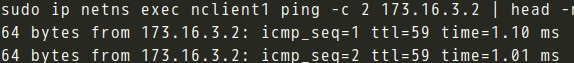
\includegraphics[width=0.8\textwidth]{figs/c1-s4-ping.jpeg}\\
    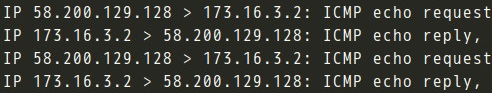
\includegraphics[width=0.8\textwidth]{figs/c1-s4-pdump.jpeg}
    \caption{基于源地址的调度}
  \end{figure}

  \vspace{-1em}

  \begin{figure}
    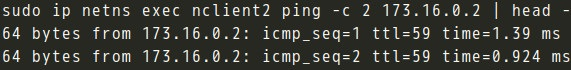
\includegraphics[width=0.8\textwidth]{figs/c2-s1-ping.jpeg}\\
    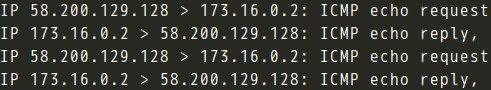
\includegraphics[width=0.8\textwidth]{figs/c2-s1-pdump.jpeg}
    \caption{基于目的地址的调度}
  \end{figure}
\end{frame}

\begin{frame}
  \frametitle{实验平台}

  \begin{center}
    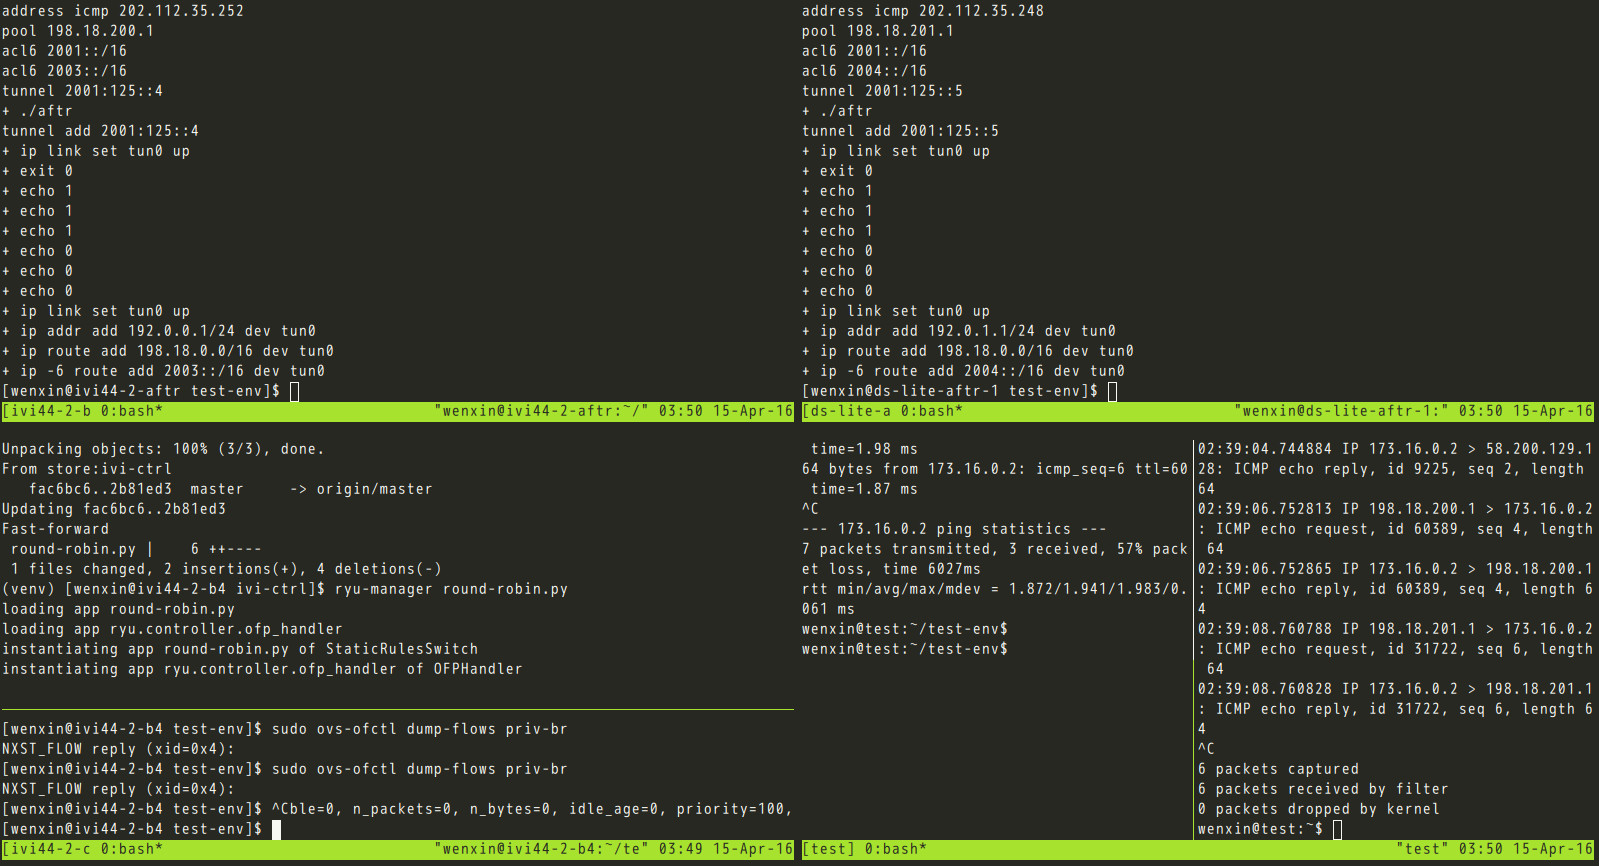
\includegraphics[width=\textwidth]{figs/test-env.jpeg}
  \end{center}
\end{frame}

\section{总结}
\begin{frame}
  \frametitle{总结和计划}

  \begin{block}{总结}
    \begin{itemize}
    \item 设计调度机制,使得过渡场景下的流量调度成为可能
      \begin{itemize}
      \item 与具体过渡技术解耦的(通用),基于五元组(灵活)
      \end{itemize}
    \item 扩展过渡技术,符合多出口场景的需求
    \end{itemize}
  \end{block}

  \begin{block}{后续工作}
    \begin{itemize}
    \item 在实际场景中测试,获取性能指标
    \item 利用调度机制研发流量调度应用解决实际需求
    \end{itemize}
  \end{block}
\end{frame}

\section{参考文献}
\begin{frame}
  \frametitle{参考文献}
  \begin{itemize}
  \item \href{https://tools.ietf.org/html/rfc7599}{RFC7599}
  \item \href{https://tools.ietf.org/html/rfc7597}{RFC7597}
  \item \href{https://tools.ietf.org/html/rfc6219}{RFC6219}
  \item \href{https://tools.ietf.org/html/rfc6052}{RFC6052}
  \item \href{https://tools.ietf.org/html/rfc7598}{RFC7598}
  \item \href{http://www.netfilter.org}{The netfilter.org project}
  \end{itemize}
\end{frame}

\section{Q\&A}

\begin{frame}
  \frametitle{Q\&A}
  \begin{center}
    {\LARGE 谢谢!}
    \vspace{3em}
    {\LARGE 请老师们提问和指导!}
  \end{center}
\end{frame}
\end{document}